\begin{frame}
  \frametitle{Empirical questions}

  \begin{itemize}

  \item How much data is needed for R-W learning convergence with the
    Danks equilibria

  \item Are there cases where we observe non-convergence between the
      R-W learning associations and Danks equilibria -- if yes, why?

    \item Does NDL accuracy always improve with increasing cues?
      If not, why?
      
  \end{itemize}
  
\end{frame}

\begin{frame}
  \frametitle{Non-equivocal positive assocation -- convergence}

  \includegraphics[width=8cm]{{{img/think.qitl2.AgentGroup_pohtia_RW_vs_D}}}

\end{frame}

\begin{frame}
  \frametitle{Non-equivocal positive association -- convergence with 1x data}

  \includegraphics[width=8cm]{{{img/think.qitl2.PersonFirst_miettia_RW_vs_D}}}

\end{frame}

\begin{frame}
  \frametitle{Non-equivocal negative association -- convergence with 1x data}

  \includegraphics[width=8cm]{{{img/think.qitl2.PersonFirst_pohtia_RW_vs_D}}}

\end{frame}

\begin{frame}
  \frametitle{Near-perfect positive association -- non-convergence with 1x data}

  \includegraphics[width=8cm]{{{img/think.qitl2.PatientInfinitive_ajatella_RW_vs_D}}}

\end{frame}

\begin{frame}
  \frametitle{Near-perfect negative association -- non-convergence with 1x data}

  \includegraphics[width=8cm]{{{img/think.qitl2.PatientDirectQuote_ajatella_RW_vs_D}}}

\end{frame}

\begin{frame}
  \frametitle{Near-perfect positive association -- convergence with 5x data}

  \includegraphics[width=8cm]{{{img/think.qitl2.PatientInfinitive_ajatella_RW_vs_Dx5}}}

\end{frame}
\begin{frame}
  \frametitle{Near-perfect negative association -- convergence with 5x data}

  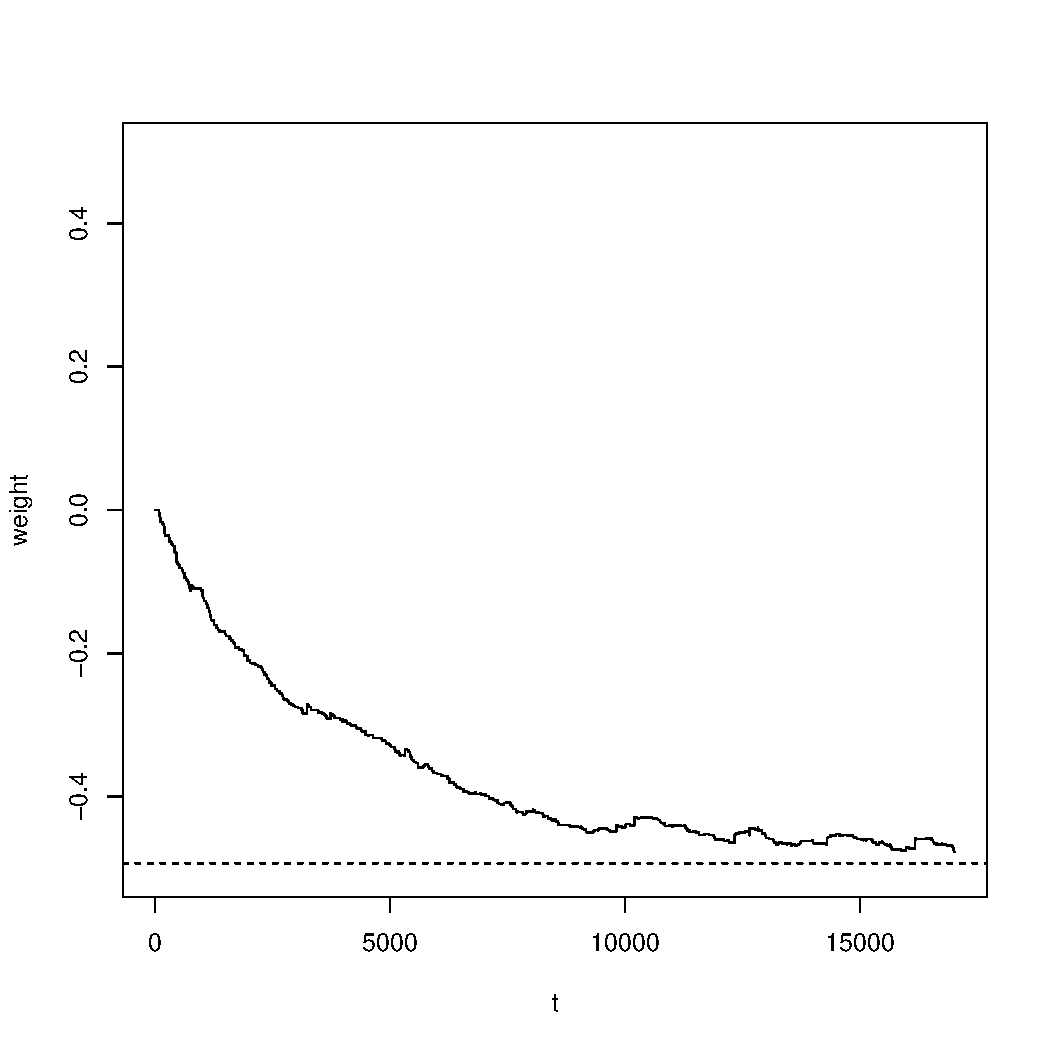
\includegraphics[width=8cm]{{{img/think.qitl2.PatientDirectQuote_ajatella_RW_vs_Dx5}}}

\end{frame}

\begin{frame}
  \frametitle{Convergence vs. non-convergence -- artificial data: plurals}

  \begin{table}[h]
    \begin{tabular}{ l | r | r | r }
      
 WordForm & Frequency &   Outcomes &     Cues \\
 hand &       10 &    hand\_NIL &   h\_a\_n\_d \\
 hands &       20 & hand\_PLURAL & h\_a\_n\_d\_s \\
 land &        8 &    land\_NIL &   l\_a\_n\_d \\
 lands &        3 & land\_PLURAL & l\_a\_n\_d\_s \\
 and &       35 &     and\_NIL &     a\_n\_d \\
 sad &       18 &     sad\_NIL &     s\_a\_d \\
 as &       35 &      as\_NIL &       a\_s \\
 lad &      102 &     lad\_NIL &     l\_a\_d \\
 lad &       54 &  lad\_PLURAL &     l\_a\_d \\
 lass &      134 &    lass\_NIL &   l\_a\_s\_s \\

    \end{tabular}
    \end{table}
  
    \end{frame}

\begin{frame}
  \frametitle{Perfect association -- convergence}

\includegraphics[width=8cm]{{{img/plurals_h_hand}}}

\end{frame}

\begin{frame}
  \frametitle{Non-equivocal positive association -- non-convergence}

  \includegraphics[width=8cm]{{{img/plurals_s_PLURAL}}}

\end{frame}

\begin{frame}  \frametitle{Non-equivocal positive association -- convergence}

  \includegraphics[width=8cm]{{{img/plurals_a_as}}}

\end{frame}

\begin{frame}
  \frametitle{Non-equivocal negative association -- non-convergence}

  \includegraphics[width=8cm]{{{img/plurals_s_as}}}

\end{frame}

%%% Local Variables: 
%%% mode: latex
%%% TeX-master: "../qitl6_evert_arppe"
%%% End: 
